\documentclass[a4paper,titlepage,11pt]{article}
\usepackage{a4wide}
\usepackage{fullpage}
\usepackage[utf8x]{inputenc}
\usepackage[slovene]{babel}
\selectlanguage{slovene}
\usepackage[toc,page]{appendix}
\usepackage[pdftex]{graphicx} % za slike
\usepackage{setspace}
\usepackage{color}
\usepackage{amsmath}
\usepackage[table]{xcolor}
\usepackage{tabularx}
\usepackage{float}
\usepackage{hhline}
\definecolor{light-gray}{gray}{0.95}
\usepackage{listings} % za vključevanje kode
\usepackage{hyperref}
\renewcommand{\baselinestretch}{1.2} % za boljšo berljivost večji razmak
\renewcommand{\arraystretch}{1.2}
\hyphenpenalty=10000
\newcolumntype{Y}{>{\centering\arraybackslash}X}
\usepackage[font=small, skip=11pt, hypcap=true]{caption}
\usepackage{indentfirst}
\setlength{\parskip}{11pt}
\usepackage{multirow}

\title{Temperaturna plošča}
\author{Rok Grmek, Matej Klemen}
\date{3. november 2017}

\begin{document}

\maketitle

\tableofcontents
\pagebreak

\section*{Uvod}

V okviru predmeta Porazdeljeni sistemi rešujeva problem temperaturne plošče. Na tem problemu bova tekom semestra spoznavala različne pristope za paralelno programiranje.

Problem temperaturne plošče je predstavljen s ploščo, ki je na treh straneh (zgoraj, levo in desno) segreta na 100 °C, na spodnji stranici pa ohlajena na 0 °C. Zanima nas, kako se v takem primeru toplota porazdeli po plošči (primer porazdelitve temperature je viden na sliki \ref{primer-temperaturne-plosce}).

\begin{figure}[H]
\begin{center}

\includegraphics[scale=0.6]{primer-temperaturne-plosce.png}
\caption{Primer temperaturne plošče, kjer rdeča barva prikazuje najvišjo, temno modra barva pa najnižjo temperaturo.}
\label{primer-temperaturne-plosce}
\end{center}
\vspace{-25pt}
\end{figure}

Iskala bova stacionarno rešitev enačbe \(\nabla^2 W = f(x, y)\), pomagala pa si bova z metodo končnih diferenc. Ploščo bova najprej razdelila na mrežo točk in posameznim točkam določila začetne vrednosti. Nato bova v vsaki točki izračunala novo temperaturo na podlagi sosednjih točk. Postopek računanja novih točk se bo ponavljal, dokler rešitev ne skonvergira.

\pagebreak

\section{Serijski algoritem}

\subsection{Opis implementacije}

Program ima dva načina delovanja. Če je definirana vrednost \textit{TIME\_MEASUREMENTS}, se bo program za podane argumente večkrat izvedel in izračunal nekaj uporabnih statistik. Ta način je namenjen predvsem opazovanju časa izvajanja programa. Sicer pa se bo program izvedel 1-krat in na koncu vizualiziral porazdelitev temperature na plošči. V nadaljevanju je opisan slednji način izvajanja, celotno delovanje programa pa je predstavljeno tudi z diagramom zaporedja, vidnim na sliki \ref{diagram-zaporedja}.

\begin{figure}[H]
\begin{center}
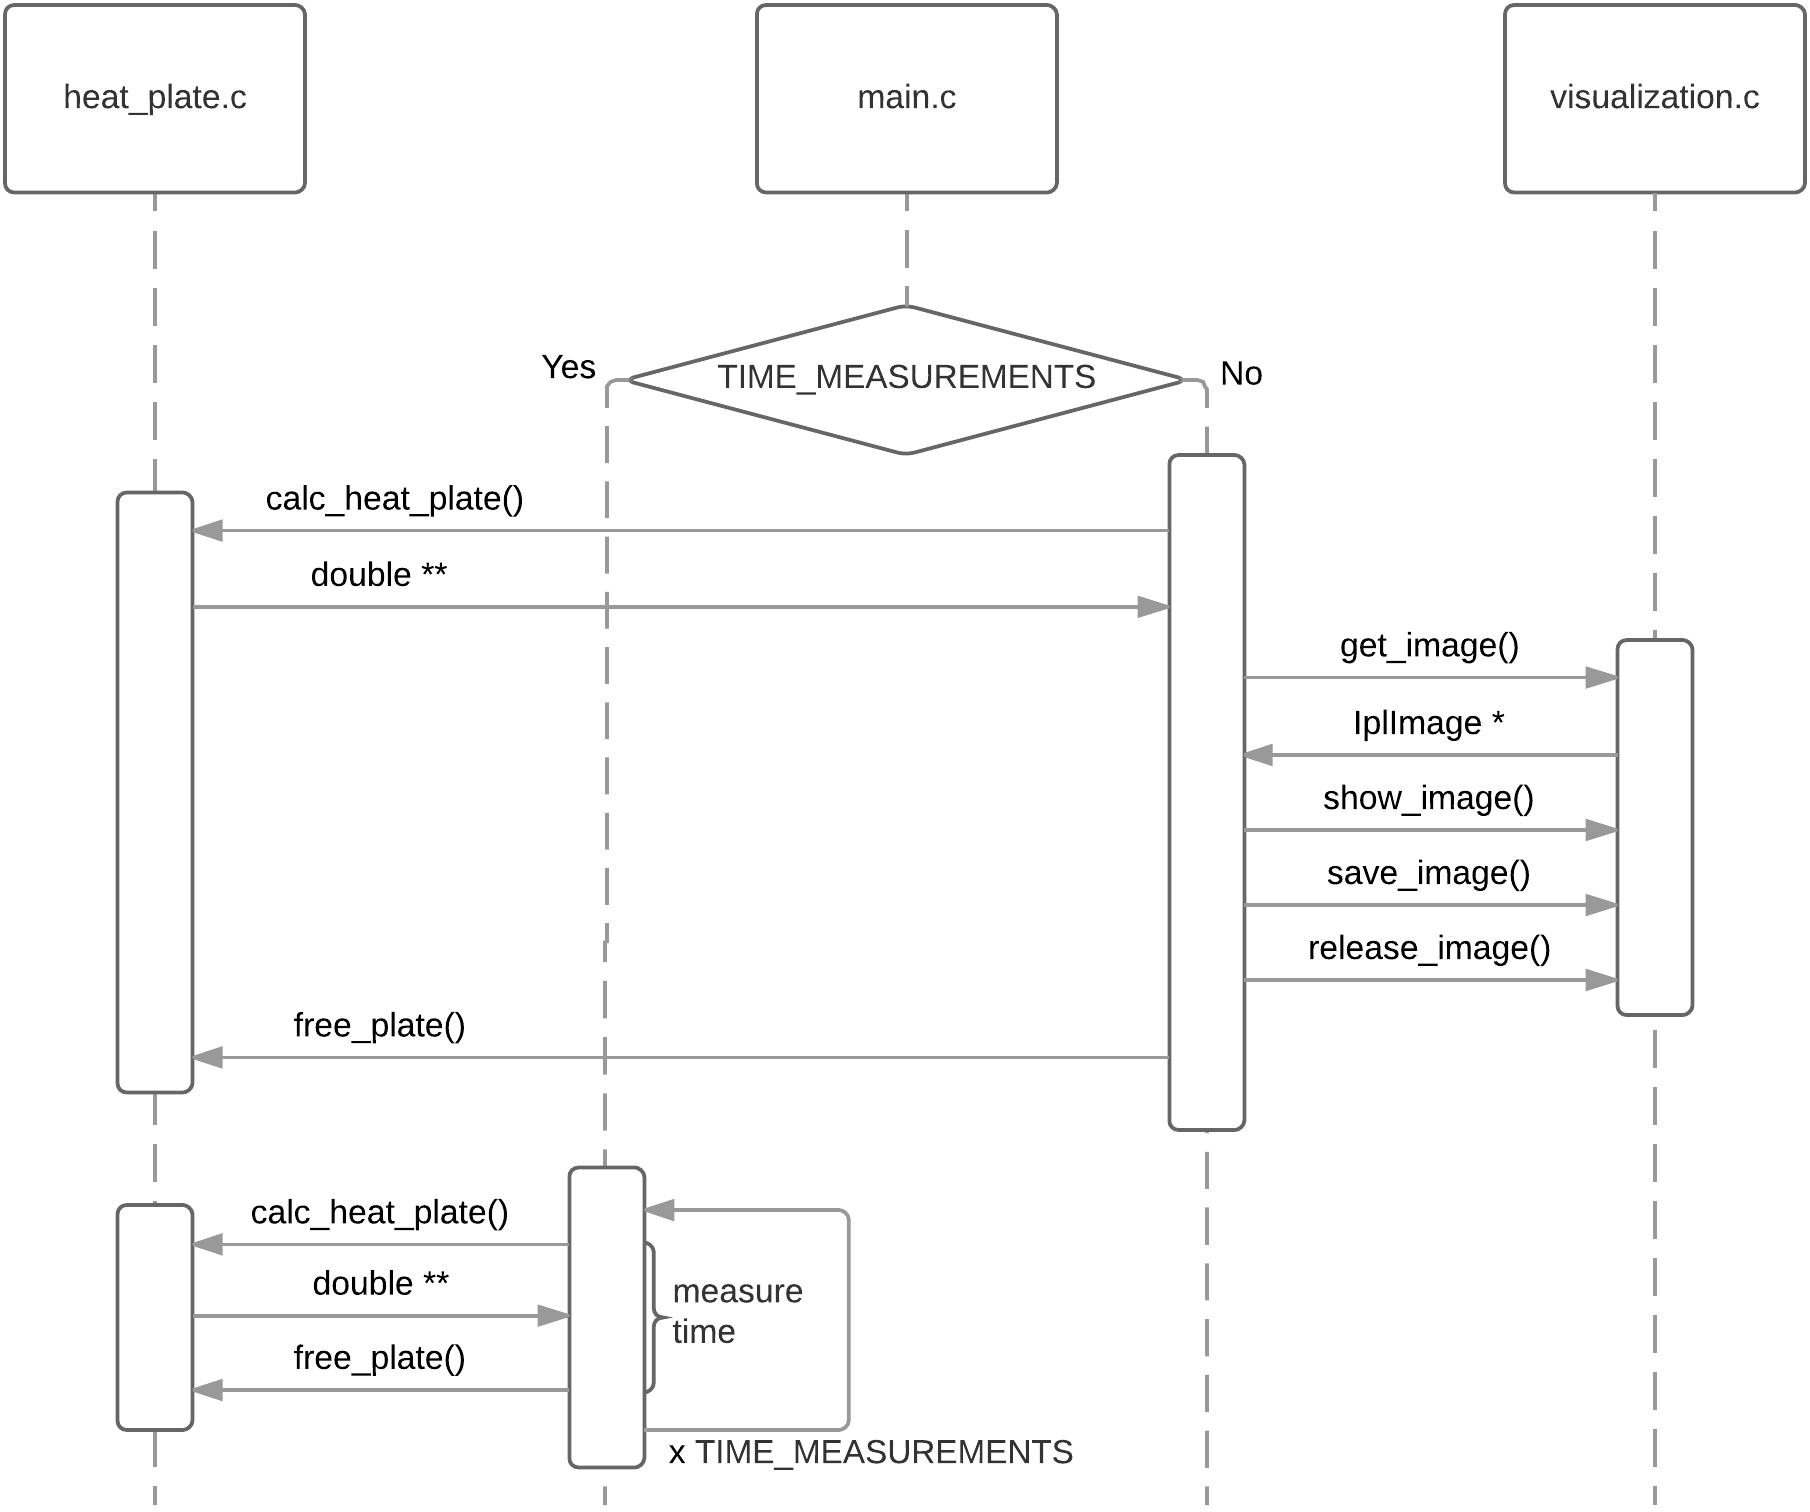
\includegraphics[scale=0.8]{diagram-zaporedja.png}
\caption{Diagram zaporedja, ki prikazuje delovanje programa.}
\label{diagram-zaporedja}
\end{center}
\vspace{-25pt}
\end{figure}

Algoritem sprejme 3 argumente: višino plošče, širino plošče in mejno razliko med dvema iteracijama (v nadaljevanju označeno z \(\varepsilon\)), na podlagi katere se zaključi računanje. Plošči, ki jo določata vnešena višina in širina, algoritem na vseh štirih stranicah doda pas širine 1, ki služi za nastavljanje robnega pogoja temperature. Novi dimenziji sta torej:
\begin{equation}
vi\breve{s}ina := vi\breve{s}ina + 2
\end{equation}
\begin{equation}
\breve{s}irina := \breve{s}irina + 2
\end{equation}
Na začetku se alocirata dve tabeli dimenzij $ vi\breve{s}ina \times \breve{s}irina$. Ena predstavlja trenutno stanje plošče, druga pa stanje plošče v prejšnji iteraciji. Alokaciji sledi inicializacija plošče - trem stranicam (levi, desni, zgornji) algoritem nastavi temperaturo na 100 °C, eni (spodnji) pa na 0 °C. Vsem ostalim celicam plošče se zaporedno (\textit{od zgoraj navzdol, od leve proti desni}) dodeli povprečje leve sosednje, zgornje sosednje, povsem desne ter povsem spodnje celice plošče. Eno izmed plošč algoritem izbere kot ploščo trenutnega, drugo pa kot ploščo prejšnjega stanja.
\indent \par Nato sledi glavna zanka. V vsaki iteraciji gre algoritem skozi ``dinamične'' celice plošče (celice, ki niso del katerega izmed robov plošče) in za vsako tako celico c[i][j] v \textit{i}-ti vrstici in \textit{j}-tem stolpcu po naslednji formuli izračuna novo temperaturo:
\begin{equation}
c[i][j] := \frac{c'[i - 1][j] + c'[i][j - 1] + c'[i][j + 1] + c'[i + 1][j]}{4},
\end{equation}
kjer $c'[i][j]$ predstavlja temperaturo celice v \textit{i}-ti vrstici in \textit{j}-tem stolpcu v prejšnji iteraciji. Ob vsakem izračunu nove temperature algoritem izračuna še absolutno razliko med trenutno (novo) in prejšnjo temperaturo ter jo v primeru, da je to v trenutni iteraciji največja izračunana absolutna razlika temperatur, shrani. Ob koncu iteracije algoritem zamenja vlogi plošč (tista, ki je do sedaj predstavljala prejšnje stanje plošče, bo v naslednji iteraciji vsebovala novo stanje plošče in obratno), pred prehodom v naslednjo iteracijo pa preveri, če je temperaturna razlika v tej iteraciji že manjša od \(\varepsilon\) (v takem primeru se računanje zaključi).

Na koncu algoritem izpiše število izvedenih iteracij in zažene vizualizacijo končnega stanja temperaturne plošče. O vizualizaciji temperaturne plošče pa je več napisano v naslednjem poglavju.

\subsection{Uporabljene knjižnice} \label{section-uporabljene-knjiznice}

Za vizualizacijo temperaturne plošče uporabljava knjižnico \textit{OpenCV}. Najprej se pripravi prazna slika (\textit{cvCreateImage}) z dimenzijami naše plošče, nato pa se za vsako točko na plošči pretvori temperaturo v 3 8-bitne kanale (rdeča, zelena, modra) in vrednosti prepiše na sliko. Če slika z največjo stranico presega \textit{MAX\_SIZE}, potem se jo še pomanjša (\textit{cvResize}). Pripravljeno sliko se prikaže (\textit{cvShowImage}) v oknu (\textit{cvNamedWindow}, \textit{cvMoveWindow}, \textit{cvResizeWindow}) in shrani na disk (\textit{cvSaveImage}). Na koncu se le še sprosti zaseden pomnilnik (\textit{cvReleaseImage}). Primer vizualizacije je viden na sliki \ref{primer-temperaturne-plosce}.

\subsection{Rezultati}

Program je bil testiran na sistemu, katerega specifikacije so navedene v tabeli \ref{tabela-specifikacije}. Da bi k izmerjenemu času čim manj pripomogli stroški režije operacijskega sistema, je bil sistem med testiranjem minimalno obremenjen z drugimi procesi.
\begin{table}[H]
\begin{center}
\caption{Specifikacije testnega sistema.}
\label{tabela-specifikacije}
\begin{tabularx}{\textwidth}{|YY|}
\hhline{==}
Procesor: & Intel Core i5-4210U\tabularnewline
Frekvenca procesorja: & 1.70GHz \tabularnewline
Število jeder: & 2 \tabularnewline
Maksimalno število niti: & 4 \tabularnewline
Velikost predpomnilnika: & 3MB \tabularnewline
Velikost in tip glavnega pomnilnika: & 16GB DDR3 \tabularnewline
Grafična kartica: & NVIDIA GeForce 820M 2GB DDR3 \tabularnewline
Operacijski sistem: & Ubuntu 16.04 \tabularnewline
\hhline{==}
\end{tabularx}
\end{center}
\vspace{-25pt}
\end{table}

Pri testiranju sva se omejila na fiksno vrednost \(\varepsilon = 0,01\) in na plošče kvadratne oblike, spreminjala pa sva zgolj velikost stranice. Za vsako izbrano velikost sva algoritem 100-krat zagnala in vsakič izmerila čas izvajanja. Iz meritev sva nato izračunala povprečni čas izvajanja in standardno napako (ta predstavlja razpršenost meritev okrog povprečnega časa). Rezultati so navedeni tabelarično v tabeli \ref{tabela-rezultati-1} in z grafom, prikazanim na sliki \ref{graf-rezultati-1}.

\begin{table}[H]
\begin{center}
\caption{Povprečni čas izvajanja programa in standardna napaka v odvisnosti od velikosti stranice.}
\label{tabela-rezultati-1}
\begin{tabularx}{\textwidth}{|YYY|}
\hhline{===}
Velikost stranice [št. točk] & Povprečni čas izvajanja [s] & Standardna napaka [s] \tabularnewline
\hhline{===}
100 & 0,250 & 0,000 \tabularnewline
200 & 0,965 & 0,001 \tabularnewline
400 & 3,877 & 0,003 \tabularnewline
800 & 15,516 & 0,006 \tabularnewline
1600 & 62,272 & 0,062 \tabularnewline
\hhline{===}
\end{tabularx}
\end{center}
\vspace{-25pt}
\end{table}

\begin{figure}[H]
\begin{center}
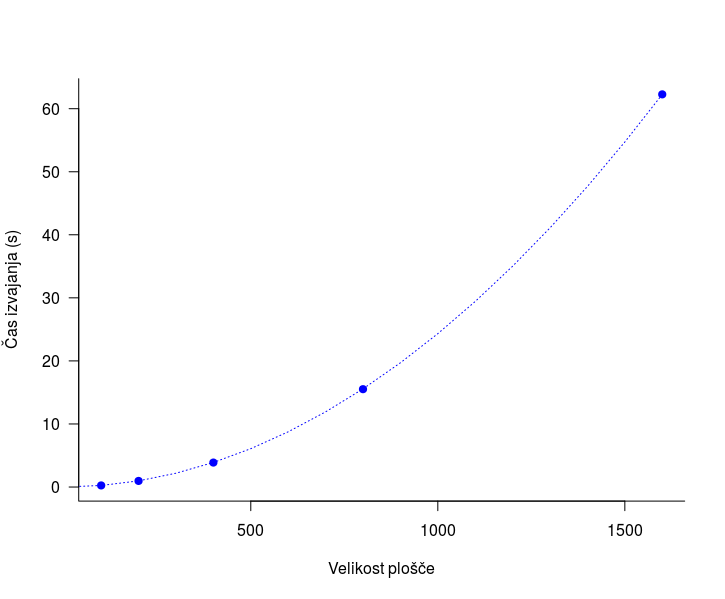
\includegraphics[scale=0.54]{graf-rezultati-1.png}
\caption{Graf, ki prikazuje povprečni čas izvajanja programa v odvisnosti od velikosti stranice.}
\label{graf-rezultati-1}
\end{center}
\vspace{-25pt}
\end{figure}

Iz rezultatov je vidno, da je povprečni čas izvajanja kvadratno odvisen od velikosti stranice plošče, kar ustreza tudi teoretični časovni zahtevnosti \(O(k \cdot h \cdot w)\), kjer je \textit{k} število iteracij, \textit{h} višina, \textit{w} pa širina plošče. V našem primeru je namreč število iteracij konstantno (določeno z \(\varepsilon\)) in velja zveza \(h=w\). Točke na grafu se zelo lepo prilegajo funkciji \(t(x) = 2,432 \cdot 10^{-5} \cdot x^{2}\), iz te pa lahko razberemo, da algoritem na testnem sistemu potrebuje približno \(2,432 \cdot 10^{-5}\) s za izračun posamezne točke (v vseh iteracijah skupaj).

\pagebreak

\section{Paralelizacija s knjižnico ``Pthreads''}

\subsection{Ideja paralelizacije} \label{ideja-paralelizacije-pthreads}

Do vključno inicializacije plošč poteka vse enako kot v serijskem algoritmu, za tem pa se delo razdeli med \textit{NUM\_THREADS} niti. Vsaka nit v posamezni iteraciji izračuna svoj delež vrstic. Pred računanjem se meje vrstic določijo na podlagi spodnjih enačb (\textit{index} predstavlja zaporedno številko niti iz intervala $\left[0, NUM\_THREADS - 1\right]$, ki jo dobi posamezna nit podano kot argument).
\begin{equation}
spodnja \ meja := 1 + \left \lfloor{\frac{index \cdot (h - 2)}{NUM\_THREADS}}\right \rfloor
\end{equation}
\begin{equation}
zgornja \ meja := 1 + \left \lfloor{\frac{(index+1) \cdot (h - 2)}{NUM\_THREADS}}\right \rfloor
\end{equation}
V zgornjih enačbah $(h - 2)$ predstavlja število vrstic, katerih temperatura ni fiksno nastavljena. Te razdeliva kar se da enakomerno med niti, na koncu pa mejam še prištejeva 1, saj je temperatura prve vrstice fiksno nastavljena na 100 °C in se računanje začne v drugi vrstici. V takem primeu delitve se število dodeljenih vrstic med posamenzimi nitmi razlikuje za kvečjemu eno vrstico.

Ko niti poračunajo svoj del plošče, morajo počakati na preostale niti, saj je nadaljnje izvajanje programa odvisno od izračunov vseh niti v trenutni iteraciji. To je doseženo s postavitvijo t.i. prepreke (angl. \textit{barrier}), ki nitim ne pusti opravljati nadaljnjega dela, dokler vse niti ne pridejo do mesta, kjer je postavljena.

Sledi postopek sinhronizacije največje izračunane absolutne razlike temperature v trenutni iteraciji. Vsaka nit je ta podatek izračunala na svojem delu plošče in ga shranila globalno, v tem delu pa posamezna nit preveri, če so vsi izračunani lokalni maksimumi pod mejo \(\varepsilon\). V takem primeru se računanje zaključi, niti se združijo in program poteka od tu naprej enako kot pri serijskem algoritmu. V nasprotnem primeru se niti počakajo (še ena prepreka) in nato hkrati začnejo novo iteracijo.

\subsection{Rezultati}

Program je bil testiran na istem sistemu (specifikacije so navedene v tabeli \ref{tabela-specifikacije}) in pri enakih pogojih kot serijski algoritem. Za fiksno vrednost \(\varepsilon = 0,01\) sva izmerila čase pri različnih velikostih plošče in za različno število niti. Rezultati so vidni v tabeli \ref{tabela-rezultati-2} in na grafu \ref{graf-rezultati-2}.

\begin{table}[H]
\begin{center}
\caption{Povprečni čas izvajanja paralelnega programa in standardna napaka glede na velikost stranice in število uporabljenih niti z uporabo knjižnice Pthreads.}
\label{tabela-rezultati-2}
\begin{tabularx}{\textwidth}{|YYYY|}
\hhline{====}
Število uporabljenih niti & Velikost stranice [št. točk] & Povprečni čas izvajanja [s] & Standardna napaka [s] \tabularnewline
\hhline{====}
\multirow{ 5}{*}{1}
& 100 & 0,253 & 0,000 \tabularnewline
& 200 & 0,974 & 0,000 \tabularnewline
& 400 & 3,890 & 0,002 \tabularnewline
& 800 & 15,935 & 0,071 \tabularnewline
& 1600 & 62,760 & 0,052 \tabularnewline
\hline
\multirow{ 5}{*}{2}
& 100 & 0,167 & 0,002 \tabularnewline
& 200 & 0,578 & 0,006 \tabularnewline
& 400 & 2,282 & 0,020 \tabularnewline
& 800 & 9,130 & 0,044 \tabularnewline
& 1600 & 35,545 & 0,030 \tabularnewline
\hline
\multirow{ 5}{*}{3}
& 100 & 0,199 & 0,000 \tabularnewline
& 200 & 0,729 & 0,000 \tabularnewline
& 400 & 2,740 & 0,000 \tabularnewline
& 800 & 10,778 & 0,002 \tabularnewline
& 1600 & 42,850 & 0,005 \tabularnewline
\hline
\multirow{ 5}{*}{4}
& 100 & 0,163 & 0,001 \tabularnewline
& 200 & 0,558 & 0,001 \tabularnewline
& 400 & 2,149 & 0,000 \tabularnewline
& 800 & 8,557 & 0,001 \tabularnewline
& 1600 & 33,917 & 0,005 \tabularnewline
\hline
\multirow{ 5}{*}{8}
& 100 & 0,212 & 0,000 \tabularnewline
& 200 & 0,680 & 0,001 \tabularnewline
& 400 & 2,414 & 0,001 \tabularnewline
& 800 & 8,874 & 0,003 \tabularnewline
& 1600 & 34,636 & 0,023 \tabularnewline
\hline
\hhline{====}
\end{tabularx}
\end{center}
\vspace{-25pt}
\end{table}

\begin{figure}[H]
\begin{center}
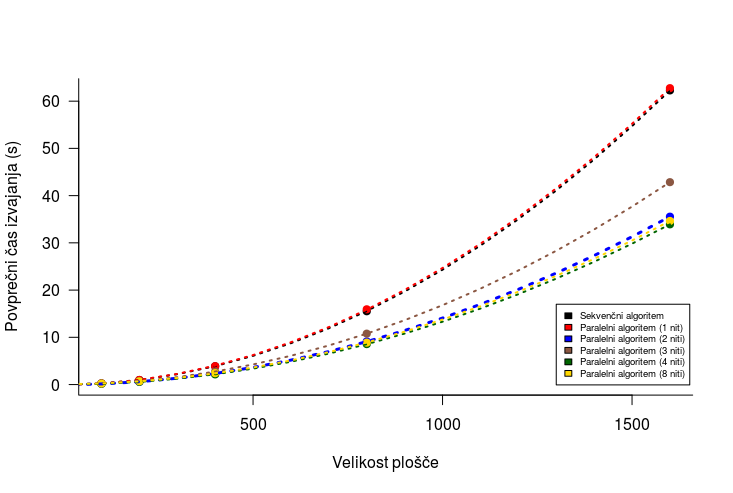
\includegraphics[scale=0.55]{graf-rezultati-2_1.png}
\caption{Povprečni čas izvajanja paralelnega programa glede na velikost plošče ob uporabi različnega števila niti (Pthreads).}
\label{graf-rezultati-2}
\end{center}
\vspace{-25pt}
\end{figure}

Za lažjo analizo meritev definiramo \textbf{faktor pohitritve} $S$ kot:
\begin{equation}
S = \frac{T_s}{T_p},
\end{equation}
kjer je $T_s$ čas izvajanja sekvenčnega programa, $T_p$ pa čas izvajanja paralelnega programa.
Največja dosežena pohitritev je bila 1,813-krat in sicer v primeru štirih niti (toliko je tudi logičnih jeder na testnem sistemu). Ta pohitritev je sicer le malo boljša od tiste v primeru dveh niti, ampak je tak rezultat pričakovan, saj imamo le dve fizični jedri. ``Hyper-threading'' nam ne prinese bistvene pohitritve, saj je naše računanje zahtevno tudi iz vidika pomnilniških dostopov, tukaj pa si po dve niti delita isti predpomnilnik. V primeru še večjega števila niti nam faktor pohitritve celo pada, saj čas izvajanja še narašča zaradi režije in preklapljanja med nitmi, hkrati pa že izkoriščamo vse razpoložljive vire sistema. To je vidno tudi na grafu \ref{graf-rezultati-pohitritev}.

\begin{figure}[H]
\begin{center}
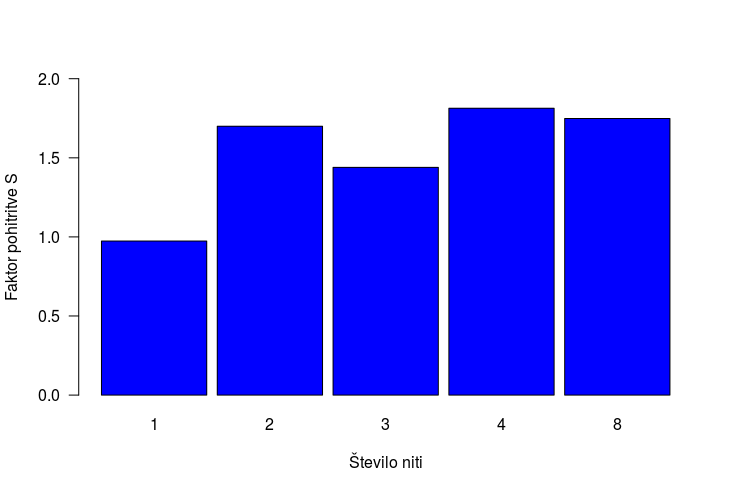
\includegraphics[scale=0.5]{graf-rezultati-2_2.png}
\caption{Faktor pohitritve v odvisnosti od števila uporabljenih niti za fiksno velikost plošče 800$\times$800 (Pthreads).}
\label{graf-rezultati-pohitritev}
\end{center}
\vspace{-25pt}
\end{figure}

Smiselno je preveriti še \textbf{učinkovitost} oziroma izkoristek uporabljenih niti, $E$, ki jo izračunamo kot:
\begin{equation}
E = \frac{S_N}{N},
\end{equation}
kjer je $S_N$ faktor pohitritve in $N$ število niti. Učinkovitost je najboljša v primeru ene same niti (0,974). Rahlo slabšo a še vedno zadovoljivo učinkovitost dosežemo tudi za dve niti (0,849), pri večjem številu niti pa ta precej pade, saj smo omejeni na zgolj dve fizični jedri. Učinkovitost v odvisnosti od števila niti je vidna na grafu \ref{graf-rezultati-ucinkovitost}.

\begin{figure}[H]
\begin{center}
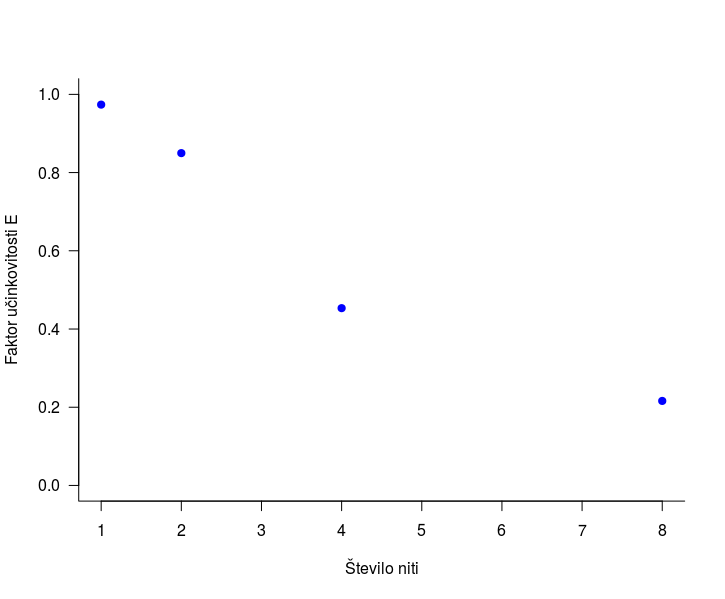
\includegraphics[scale=0.5]{graf-rezultati-2_3.png}
\caption{Učinkovitost v odvisnosti od števila uporabljenih niti za fiksno velikost plošče 800$\times$800 (Pthreads).}
\label{graf-rezultati-ucinkovitost}
\end{center}
\vspace{-25pt}
\end{figure}

\pagebreak

\section{Paralelizacija s knjižnico ``OpenMP''}

\subsection{Ideja paralelizacije}
Paralelizacija poteka na podoben način kot paralelizacija s knjižnico Pthreads (za katero je ideja paralelizacije opisana v poglavju \ref{ideja-paralelizacije-pthreads}). Na začetku vsake iteracije se delo statično razdeli med vse niti - vsaka nit dobi $\frac{\breve{s}tevilo \ vrstic \ - \ 2}{\breve{s}tevilo \ niti}$ vrstic. Če $\breve{s}tevilo \ vrstic \ - \ 2$ ni deljivo s $\breve{s}tevilo \ niti$ (ostane $0 < r < \breve{s}tevilo \ niti$), potem se prvim $r$ nitim dodeli še po 1 vrstico.

Zatem vsaka nit poračuna svoj del plošče, na koncu pa niti sinhronizirajo maksimalne absolutne razlike med starimi in novimi temperaturami, ki so jih izračunale na svojem delu plošče v trenutni iteraciji. Če je največja izmed teh temperatur manjša od meje konvergence $\varepsilon$, se izračun konča, sicer pa se začne nova iteracija in ponovi postopek.

V primerjavi s paralelizacijo s knjižnico Pthreads je bilo tukaj potrebno manj dela. Če zanemarimo vključevanje knjižnice OpenMP in nastavitev števila niti, ki jih program uporablja, je bila paralelizacija dosežena zgolj z naslednjo vrstico:
\begin{lstlisting}
#pragma omp parallel for reduction(max: max_diff).
\end{lstlisting}
To navodilo prevajalniku pove, naj poskrbi, da se delo porazdeli tako, kot je bilo navedeno v prvem odstavku tega poglavja ter da se niti na koncu počakajo in sinhronizirajo svoje lokalne podatke.

\subsection{Rezultati}

Program je bil testiran na sistemu, opisanem v tabeli \ref{tabela-specifikacije}. \\
Izmerjeni časi so zelo podobni časom, izmerjenim na programu, ki je bil paraleliziran s knjižnico Pthreads. 
Največjo pohitritev program doseže z uporabo štirih niti, saj ima sistem štiri fizična jedra. A ta pohitritev še zdaleč ni štirikratna, kot bi bilo pričakovati v idealnem primeru (tudi tokrat tehnologija ``Hyper-threading'' ni prinesla bistvene pohitritve). \\
Podobni rezultati so bili pričakovani, saj sta ideji paralelizacije pri obeh knjižnicah skoraj enaki - minimalna razlika se pojavi zgolj pri delitvi dela med nitmi. Poleg tega je lahko minimalni časovni pribitek ali pa odbitek posledica različno učinkovitih implementacij paralelnih konstruktov v posamezni knjižnici.


\textbf{TODO} (dopolni) komentar rezultatov, grafi rezultatov, primerjava s Pthreads

\begin{table}[H]
\begin{center}
\caption{Povprečni čas izvajanja paralelnega programa in standardna napaka glede na velikost stranice in število uporabljenih niti z uporabo knjižnice OpenMP.}
\label{tabela-rezultati-3}
\begin{tabularx}{\textwidth}{|YYYY|}
\hhline{====}
Število uporabljenih niti & Velikost stranice [št. točk] & Povprečni čas izvajanja [s] & Standardna napaka [s] \tabularnewline
\hhline{====}
\multirow{ 5}{*}{1}
& 100 & 0,253 & 0,000 \tabularnewline
& 200 & 0,973 & 0,000 \tabularnewline
& 400 & 3,983 & 0,007 \tabularnewline
& 800 & 15,808 & 0,021 \tabularnewline
& 1600 & 62,756 & 0,038 \tabularnewline
\hline
\multirow{ 5}{*}{2}
& 100 & 0,146 & 0,000 \tabularnewline
& 200 & 0,554 & 0,000 \tabularnewline
& 400 & 2,508 & 0,025 \tabularnewline
& 800 & 8,798 & 0,001 \tabularnewline
& 1600 & 35,274 & 0,002 \tabularnewline
\hline
\multirow{ 5}{*}{3}
& 100 & 0,184 & 0,000 \tabularnewline
& 200 & 0,690 & 0,000 \tabularnewline
& 400 & 2,913 & 0,001 \tabularnewline
& 800 & 10,982 & 0,018 \tabularnewline
& 1600 & 43,008 & 0,069 \tabularnewline
\hline
\multirow{ 5}{*}{4}
& 100 & 0,140 & 0,000 \tabularnewline
& 200 & 0,539 & 0,000 \tabularnewline
& 400 & 2,148 & 0,001 \tabularnewline
& 800 & 8,734 & 0,006 \tabularnewline
& 1600 & 34,699 & 0,006 \tabularnewline
\hline
\multirow{ 5}{*}{8}
& 100 & 0,193 & 0,001 \tabularnewline
& 200 & 0,643 & 0,001 \tabularnewline
& 400 & 2,284 & 0,002 \tabularnewline
& 800 & 9,025 & 0,002 \tabularnewline
& 1600 & 35,343 & 0,105 \tabularnewline
\hhline{====}
\end{tabularx}
\end{center}
\vspace{-25pt}
\end{table}

\begin{figure}[H]
\begin{center}
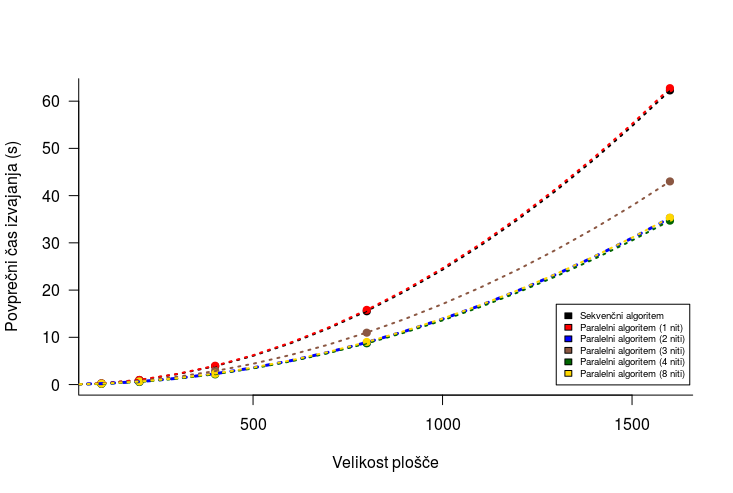
\includegraphics[scale=0.6]{graf-rezultati-3_1.png}
\caption{Povprečni čas izvajanja paralelnega programa glede na velikost plošče ob uporabi različnega števila niti (OpenMP).}
\label{graf-rezultati-3}
\end{center}
\vspace{-25pt}
\end{figure}

\begin{figure}[H]
\begin{center}
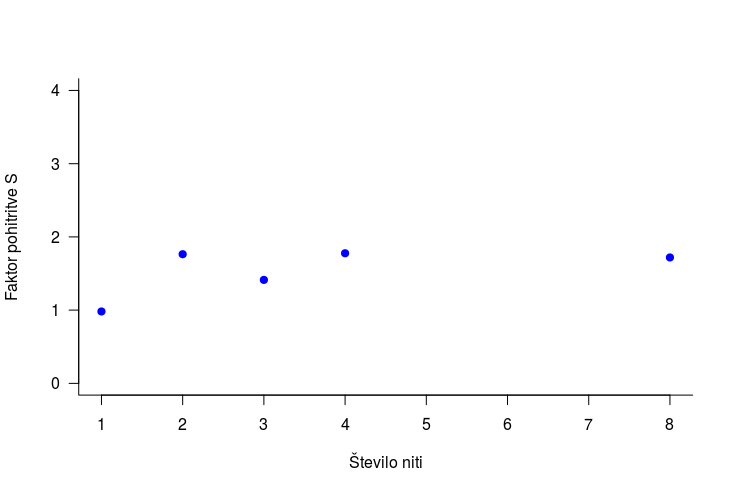
\includegraphics[scale=0.6]{graf-rezultati-3_2.png}
\caption{Faktor pohitritve v odvisnosti od števila uporabljenih niti za fiksno velikost plošče 800$\times$800 (OpenMP).}
\label{graf-rezultati-pohitritev-3}
\end{center}
\vspace{-25pt}
\end{figure}

\begin{figure}[H]
\begin{center}
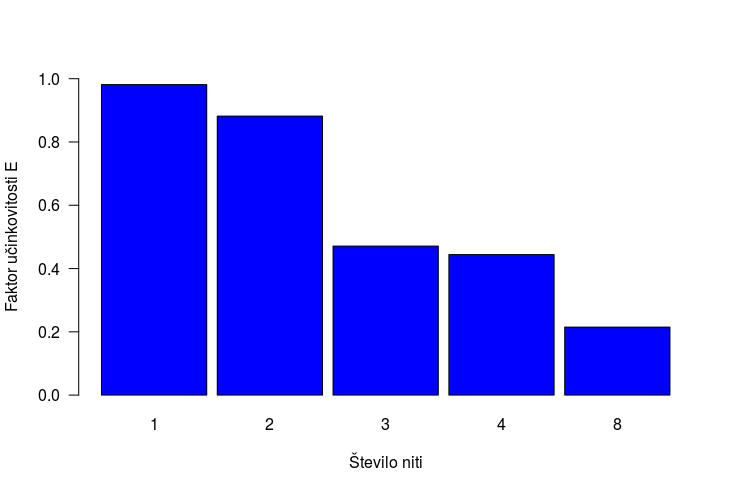
\includegraphics[scale=0.6]{graf-rezultati-3_3.png}
\caption{Učinkovitost v odvisnosti od števila uporabljenih niti za fiksno velikost plošče 800$\times$800 (OpenMP).}
\label{graf-rezultati-ucinkovitost-3}
\end{center}
\vspace{-25pt}
\end{figure}

\end{document}
